\documentclass[12pt,a4paper]{article}
\usepackage[utf8]{inputenc}
\usepackage[english]{babel}
\usepackage{amsmath}
\usepackage{amsfonts}
\usepackage{amssymb}
\usepackage{soul, color}
\usepackage{graphicx}
\usepackage{verbatim}
\usepackage{physics}
\usepackage{breqn}
\usepackage[margin=1in]{geometry}

\usepackage[
backend=biber,
style=alphabetic,
sorting=ynt
]{biblatex}

\begin{document}
\title{Lubensky Lab Vertex Model Tutorial 3}
\author{Avik Mondal}
\maketitle{}

\section{Introduction}

This tutorial assumes that you are familiar with the basics of the vertex model - by this point, hopefully you have played around with Microsoft Visual Studios (or whatever IDE you have chosen to use), run the base vertex model, and tried your hand at creating the new subclass (see "Lubensky Lab Vertex Model Tutorial 2 V2.0"). The curious reader might have wondered where choices about the  specific parameters added to the modified energy came from. In this tutorial, I will attempt to justify picking those parameters. Additionally, I will go into more details about the different ways we can create initial packings for the vertex model and different important details that are good to note before playing around with the vertex model. Note that while I have labeled sections in this document as "Chapter," I'm not trying to make you read a whole book on this.

\section{Modified Energy}
In the last tutorial, we got some practice extending the base vertex model by implementing a common variant of the energy function:

\begin{center}
\begin{equation}
\label{Perimetervariant}
E =  \sum_{\text{cells} \hspace{1mm} i} \frac{K}{2} (A_i - A_0)^2 + \frac{\Lambda}{2} (P_i - P_0)^2 + \sum_{\text{edges} \hspace{1mm} j} \gamma_0 l_j
\end{equation}
\end{center}

As the tutorial and Meryl's thesis explain, this new energy leads to a change in the edge tension:
\begin{center}
\begin{equation}
\label{edgetensions}
F = \gamma_0 + \Lambda (P_1 - P_0) + \Lambda (P_2 - P_0)
\end{equation}
\end{center}
This variant adds two new parameters to the vertex model energy: $\Lambda$ and $P_0$. This brings our total list of parameters. Going over them really quickly:

\begin{enumerate}
\item $A_0$: The preferred area term for every cell. 
\item $K$: Elastic (called "height") modulus. This gives the strength of the quadratic area term. You could also say it penalizes perturbations from the preferred area. 
\item $\gamma$:  The line tension on each edge. In this variant, it makes more sense to think of it as the interfacial tension set up by the competition between the cortical tension and cell-cell adhesion.
\item $P_0$: The preferred area term for every cell. While a preferred area term makes sense for cells (it is well known that cells can detect their own area), this term has less physical justification.
\item $\Lambda$: Penalizes variations from the preferred perimeter. Also, the term that describes the active contractility of the actin-myosin cortex. 
\end{enumerate}
There is some controversy about the validity of $P_0$ in this five parameter model. In fact, the majority of papers do not use Eqn \hspace{1mm}\ref{Perimetervariant}. A more commonly seen version of this energy is written as:
\begin{center}
\begin{equation}
\label{eqn: manningmodel1}
E_i = K (A_i - A_0)^2 + \frac{\Lambda}{2} P_i^2 + \gamma P_i
\end{equation}
\end{center}
where $E_i$ is the energy for a cell $i$. In this model, the variable definitions from the previous equation hold. The only difference is that no preferred perimeter is added. As a result, there are only 4 parameters in this model. Another interesting feature of this model is that you can write it in the form:
\begin{center}
\begin{equation}
\label{eqn: manningmodel2}
E_i = K(A_i - A_0)^2  + \frac{\Lambda}{2} (P_i - P_0)^2.
\end{equation}
\end{center}
The two equations are equivalent when you make $P_0 = -\frac{\gamma}{2 \Lambda}$. Additionally, in this model $\gamma$ can be negative. This is in stark contrast to the model that the Lubensky Lab typically uses ($\Lambda = 0$), where if $\gamma < 0$, all tensions end up negative. I refer you to \cite{1} and \cite{2} for more details (read: a better explanation) of this model. There are, of course, many more papers that will echo what these two say. I encourage you to look through them - I did not include them out of laziness (be careful to look specifically for "vertex models" and not "voronoi models," which are different). Note that Lisa Manning's group, who does also study vertex models and statistical physics/ developmental biology, studies different aspects of the field and thus uses a different regime of the vertex model's phase space for their work. To that end, I want to make it clear that I am advertising this paper because a) they succinctly give physical justifications for all their terms b) they give a better explanation for the equations \ref{eqn: manningmodel1} and \ref{eqn: manningmodel2}. 

\section{Mapping Between Models}

The reason I am writing this tutorial is because when I started Meryl's first tutorial, I found the simulation producing unphysical results for a variety of reasons. One of the major ones is that I did not know which region of phase space was good to use. Studying the model in other works helped, and here I am going to explain how I found the parameters that I recommend you use in Tutorial 2. 

I found that using Eqn \ref{eqn: manningmodel1} for the vertex model left me with far more robust packings (at least, I tried a relatively large section of phase space and no simulations broke broke). 

It is easy to see, in comparing Eqns \ref{Perimetervariant} and \ref{eqn: manningmodel2}, that you can easily map between the two models. I will show this with a simple calculation. Starting with Eqn \ref{Perimetervariant}:
\begin{center}
\begin{equation}
\begin{split}
E &=  \sum_{\text{cells} \hspace{1mm} i} \frac{K}{2} (A_i - A_0)^2 + \frac{\Lambda}{2} (P_i - P_0)^2 + \sum_{\text{edges} \hspace{1mm} j} \gamma_0 l_j\\
&=\sum_{\text{cells} \hspace{1mm} i} \frac{K}{2} (A_i - A_0)^2 + \frac{\Lambda}{2} (P_i - P_0)^2 + \frac{\gamma_0}{2} P_i\\
\end{split}
\end{equation}
\end{center}
We want to get rid of the second type of summation (over edges). Note that because we have been using confluent packings that have periodic boundary conditions, we should realize that the sum over the perimeter of all the cells is twice the sum of all the lengths of all the edges. 
\begin{center}
\begin{equation}
\begin{split}
E &= \sum_{\text{cells} \hspace{1mm} i} \frac{K}{2} (A_i - A_0)^2 + \frac{\Lambda}{2} (P_i - P_0)^2 + \frac{\gamma_0}{2} P_j\\
&= \sum_{\text{cells} \hspace{1mm} i} \frac{K}{2} (A_i - A_0)^2 +  \frac{\Lambda}{2} ( P_i^2 - 2P_i P_0 + P_0^2) + \frac{\gamma_0}{2} P_i \\
&= \sum_{\text{cells} \hspace{1mm} i} \frac{K}{2} (A_i - A_0)^2 +  \frac{\Lambda}{2} \Big[ P_i^2 - P_i \Big(2 P_0 - \frac{\gamma_0}{\Lambda} \Big) + P_0^2 \Big]  \\
& = \sum_{\text{cells} \hspace{1mm} i} \frac{K}{2} (A_i - A_0)^2 +  \frac{\Lambda}{2} \Big[ P_i - P_0' \Big]^2  \\
& = \sum_{\text{cells} \hspace{1mm} i} \frac{K}{2} (A_i - A_0)^2 +  \frac{\Lambda}{2} P_i ^2 + \Big(\frac{\gamma_0}{2} - \Lambda P_0\Big)P_i \\
\end{split}
\end{equation}
\end{center}
where $P_0' = P_0 - \frac{\gamma_0}{2 \Lambda}$. So this maps really nicely to Eqn \ref{eqn: manningmodel2}. Note, in the second to last step, we can take that step because adding constants to the energy does not affect the dynamics. The last line is just mimicking the form of Eqn \ref{eqn: manningmodel1} and dropping constants. We can then compare the "Lisa Manning" parameters to the "David Lubensky" parameters by noting that $\gamma^{\text{LM}} \rightarrow \gamma^{\text{DL}} - 2 \Lambda^{\text{DL}} P_0$, $\Lambda^{\text{LM}} \rightarrow \Lambda^{\text{DL}}$. Noting these mappings, I used the 4 parameter model to test the phase space.

\section{Phase Space Exploration}
For this exploration, I only used one fairly equilibrated, well-behaved packing (Lloyd Algorithm packings). I used parameters r = 2000, nbPoints = 20 (number of points), and limit = 30 (see Lloyd algorithm \cite{3} function to understand these parameters). I then explored $(\gamma, \Lambda)$ space. I noted two things: 1) whether the overall area of the packing shrinks and 2) whether something unphysical happens in the simulation (it "breaks"), including oscillating T1's or vertices crossing each other unphysically. Note that some of the phase points that are labelled as "breaking" do not break for the majority of the simulation (I ran the simulation for 20 seconds). 
\begin{center}
\begin{figure}[h!]
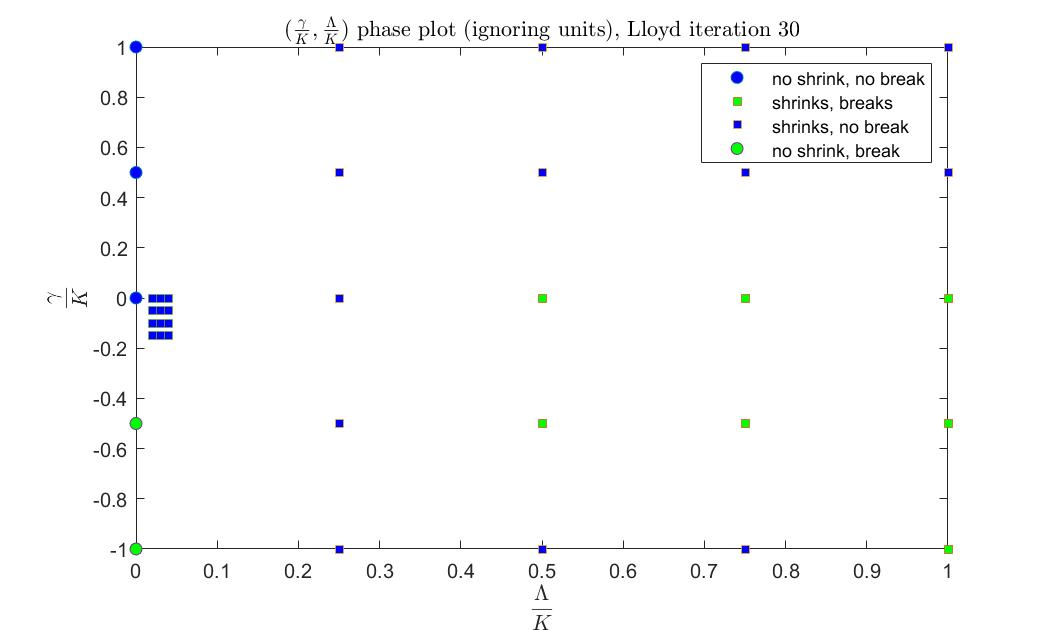
\includegraphics[scale=0.45]{phase_portrait.jpg}
\caption{Phase plot for portions of $(\gamma, \Lambda)$ phase space that don't break when using the perimeter variant of the vertex model. The coordinates shown are relative $(\frac{\gamma}{K}, \frac{\Lambda}{K})$.}
\end{figure} 
\end{center}
I ran all the simulations with $K = 10$ and plotted the ratios of $\frac{\gamma}{K}$ and $\frac{\Lambda}{K}$. I have four labels. Circles show no shrinking of the packing. Squares show shrinking. Blue points do not break and green points break. I did not spend much time coming up with physical explanations for this plot. I can say confidently that the plot breaks quickly on the $\Lambda = 0$ line as $\gamma$ decreases below $0$ because that means there are lots of negative tensions in the packings. Adding non-zero $\Lambda$ is paramount to adding a quadratic perimeter term to the mix, which usually keeps tensions positive. This falls short when you follow the $\gamma = 0$ line and see that the simulations break all along that line. My suspicion is that if I tried a larger set of packings, I would find positive $\gamma$ and positive $\Lambda$ region to be the only consistently well-behaved region of phase space. 

So mapping to the model that Meryl instructs, you can check if $\frac{\gamma}{K} - 2 \frac{\Lambda}{K} P_0$ equals one of the points corresponding to $\gamma$ in the above figure. However, you can also very quickly reprogram the code to pick whichever version of the perimeter variant you prefer. 

For those of you who are curious, I left gifs and folders of the simulations that I ran so that you can see the results. 

\section{Nice Packings}
I promised to talk about this, but there's not too much to it. Either Avik or Jakob can give you access to the function GenerationVoronoi_LloydIteration. It should also be included in the folder where all this information is. You can read up on how the Lloyd Iteration works. 
\begin{thebibliography}{9}
\bibitem{1}
Dapeng Bi, J. H. Lopez, J. M. Schwarz, and M. Lisa Manning.
\textit{A density-independent rigidity transition in biological tissues}.
(2015). \textit{Arxiv preprint}. 
\bibitem{2}
Reza Farhadifar, Jens-Christian Roper, Benoit Aigouy, Suzanne Eaton, Frank Julcher. \textit{The Influence of Cell Mechanics, Cell-Cell Interactions, and Proliferation on Epithelial Packing}. (2007). \textit{Current Biology} 17, 2095-2104. 
\bibitem{3}
Daniel Sanchez-Gutierrez, Melda Tozluoglu, Joseph D Barry, Alberto Pascual, Yanlan Mao, and Luis M Escudero. \textit{Fundamental physical cellular constraints drive self-organization of tissues}
\end{thebibliography}
\end{document}